\chapter{Cadre général du projet et démarche de résolution}
\label{chap:cadre-general}

Ce premier chapitre pose les bases du projet. Il présente le contexte professionnel du stage, décrit les deux missions confiées et justifie la démarche retenue pour les mener à bien. Nous présentons d'abord BQube ITs, l'entreprise d'accueil, puis les deux cas d'étude : le déploiement d'un \ac{LIMS} au \ac{CTAA} et la connexion des équipements de laboratoire de Pharmaghreb. Pour chacun, nous analysons l'existant et exposons la solution proposée. Nous formulons ensuite la problématique et les objectifs, avant de présenter la méthodologie et la planification du projet.

%-------------------------------------------------------------
\section{Présentation de l'entreprise d'accueil}
%-------------------------------------------------------------

Le stage s'est déroulé au sein de BQube ITs, société tunisienne de conseil et de services informatiques créée en 2017. Elle conçoit des solutions numériques destinées à l'Industrie~4.0 et accompagne les industriels et les laboratoires dans la digitalisation de leurs processus. Son savoir-faire couvre principalement :
\begin{itemize}
    \item les systèmes \ac{MES}, dédiés au pilotage de la production ;
    \item les systèmes \ac{LIMS}, dédiés à la gestion des laboratoires \citep{gibbon1996} ;
    \item le développement de logiciels sur mesure ;
    \item la numérisation des processus métier.
\end{itemize}
Ses interventions visent à renforcer, chez ses clients, la traçabilité, l'automatisation, la qualité et la gestion des données.

\begin{figure}[H]
  \centering
  
\includegraphics[width=0.45\textwidth]{logo-bqube-grand.jpg}
  \caption{Logo de la société BQube ITs.}
  \label{fig:bqube}
\end{figure}

Le projet de fin d'études s'inscrit dans cette activité à travers deux missions :
\begin{itemize}
    \item \textbf{\ac{CTAA}} : mise en place d'un \ac{LIMS} et développement d'un module de traçabilité dans un centre spécialisé dans l'analyse, le contrôle qualité et l'expertise des produits agroalimentaires ;
    \item \textbf{Pharmaghreb} : étude de la connectivité des équipements de laboratoire d'un industriel pharmaceutique, puis conception et réalisation d'un prototype d'acquisition automatique des mesures.
\end{itemize}

%-------------------------------------------------------------
\section{Premier cas d'étude : le CTAA}
%-------------------------------------------------------------

\subsection{Présentation du cas}

Le \ac{CTAA} est un organisme public tunisien fondé en 1996 \citep{ctaaweb}. Il soutient les industriels du secteur agroalimentaire par de l'assistance technique, de la formation, de la recherche et des analyses de laboratoire accréditées (microbiologie, physico-chimie, analyse sensorielle, recherche d'\ac{OGM}). Sa clientèle se compose :
\begin{itemize}
    \item des entreprises des industries alimentaires ;
    \item des opérateurs commerciaux, importateurs et exportateurs de produits alimentaires ;
    \item des organisations professionnelles, telles que la Fédération nationale de l'agroalimentaire et les chambres syndicales ;
    \item des organismes publics, principalement rattachés aux ministères chargés de l'Industrie, du Commerce, de l'Agriculture et de la Santé.
\end{itemize}

\begin{figure}[H]
  \centering
  
\includegraphics[width=0.28\textwidth]{logo-ctaa.jpg}
  \caption{Logo du Centre Technique de l'Agro-Alimentaire.}
  \label{fig:ctaa}
\end{figure}

Le laboratoire réalise des analyses physico-chimiques, microbiologiques et nutritionnelles, ce qui produit un volume important d'informations à gérer. Le traitement d'un échantillon suit un parcours en quatre étapes :
\begin{enumerate}
    \item la réception de l'échantillon et l'enregistrement de la demande ;
    \item la réalisation des analyses ;
    \item la saisie et la validation des résultats ;
    \item l'édition des rapports d'analyse.
\end{enumerate}
Chaque étape génère des données qui doivent être enregistrées, conservées et accessibles à tout moment.

Le \ac{CTAA} évolue en outre dans un cadre très exigeant en matière de qualité et de traçabilité. La norme \ac{ISO/CEI 17025}, référence internationale applicable aux laboratoires d'essais et d'étalonnage, impose au laboratoire de démontrer sa compétence et de maîtriser toutes les activités susceptibles d'influencer la validité de ses résultats \citep{iso17025}. L'enjeu principal est donc de centraliser et de structurer les informations tout en les rendant accessibles de manière sécurisée.

\subsection{Analyse de l'existant}

L'analyse de l'existant s'appuie sur des observations menées dans le laboratoire et sur des échanges avec ses utilisateurs. Elle a mis en évidence plusieurs contraintes dans la gestion des demandes, des échantillons, des analyses et des informations associées.

\subsubsection*{Volume d'activité}

Le \ac{CTAA} reçoit chaque jour entre 10 et 20 demandes d'analyses, réparties en trois catégories : les demandes d'importation, les demandes d'exportation et les demandes d'autocontrôle. Une demande porte en général sur 1 à 10 échantillons, et chaque échantillon peut nécessiter des analyses physico-chimiques, microbiologiques, ou les deux. Plusieurs intervenants doivent donc enregistrer, consulter et suivre un grand nombre de données tout au long du processus.

\subsubsection*{Identification des échantillons et limites du code-barres}

Avant le projet, les échantillons étaient identifiés par des étiquettes à code-barres linéaire (figure~\ref{fig:codebarre}). Ce mode d'identification présente plusieurs limites :
\begin{itemize}
    \item \textbf{une capacité de stockage réduite} : un code linéaire ne contient qu'une faible quantité d'informations \citep{iso15417} ;
    \item \textbf{une lecture directionnelle} : le code doit être orienté face au lecteur, ce qui ralentit l'opération ;
    \item \textbf{une sensibilité à l'impression} : une étiquette mal imprimée, abîmée ou partiellement masquée peut empêcher la lecture ;
    \item \textbf{un espace d'étiquetage limité} : les désignations longues s'affichent parfois de façon tronquée.
\end{itemize}

\begin{figure}[H]
  \centering
  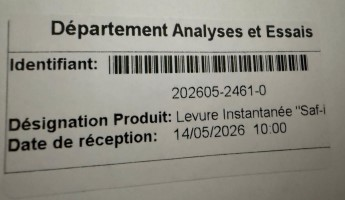
\includegraphics[width=0.42\textwidth]{etiquette-code-barres.jpg}
  \caption{Étiquette d'échantillon à code-barres utilisée avant le projet.}
  \label{fig:codebarre}
\end{figure}

\subsubsection*{Manque de centralisation et de sécurisation des données}

L'usage de plusieurs outils non intégrés entraînait une dispersion des données, des risques d'erreur lors des saisies et des difficultés pour retrouver l'information. Or la norme \ac{ISO/CEI 17025} exige de maîtriser, de tracer et de conserver correctement les informations afin d'assurer la fiabilité des résultats.

\subsubsection*{Traçabilité incomplète des opérations}

Dans un laboratoire accrédité, chaque étape du traitement d'un échantillon doit pouvoir être reconstituée, de sa réception jusqu'à la validation du résultat. L'absence de système intégré limitait la visibilité sur l'utilisateur ayant réalisé chaque opération, sur les étapes de traitement, sur l'historique des modifications et sur les équipements, réactifs et consommables utilisés.

\subsubsection*{Suivi des équipements et des compétences du personnel}

Le laboratoire doit identifier chacun de ses équipements, suivre sa maintenance et son étalonnage, et vérifier régulièrement les compétences et les habilitations de ses agents. Gérées à la main, ces informations rendent plus difficile le respect des échéances.

\subsubsection*{Délais de traitement et absence de suivi en temps réel}

La saisie sur papier et l'attente de la validation et de la signature du responsable allongeaient les délais, en particulier en période de forte activité. Faute de suivi centralisé, un client pouvait devoir revenir au \ac{CTAA} sans connaître l'état exact de sa demande.

\subsubsection*{Synthèse des problèmes identifiés}

Le tableau~\ref{tab:synthese-ctaa} résume les principaux constats et leurs conséquences.

\begin{table}[H]
\centering
\renewcommand{\arraystretch}{1.3}
\begin{tabularx}{\textwidth}{|p{5cm}|Y|}
\hline
\enteteligne \entete{Problème constaté} & \entete{Conséquence} \\ \hline
Identification par code-barres linéaire & Lecture lente ou impossible, informations tronquées \\ \hline
Données dispersées & Erreurs de saisie, recherche d'informations longue \\ \hline
Traçabilité incomplète & Historique difficile à reconstituer lors d'un audit \\ \hline
Suivi manuel des équipements et des habilitations & Échéances de maintenance, d'étalonnage et d'habilitation plus difficiles à tenir \\ \hline
Opérations manuelles et validations papier & Délais allongés, surtout en période de forte activité \\ \hline
Absence de suivi en temps réel & Déplacements et attentes inutiles pour les clients \\ \hline
\end{tabularx}
\caption{Synthèse des problèmes de l'existant au CTAA.}
\label{tab:synthese-ctaa}
\end{table}

\subsubsection*{Analyse des gaspillages selon les sept Muda}

La démarche Lean classe les pertes de temps et de ressources en sept catégories de gaspillage, appelées \emph{Muda} \citep{ohno1988,womack1996}. La figure~\ref{fig:muda} les applique au fonctionnement observé au \ac{CTAA}. Quatre d'entre elles ressortent nettement :
\begin{itemize}
    \item \textbf{l'attente} : délais de validation, de signature et de disponibilité des résultats ;
    \item \textbf{les mouvements inutiles} : clients obligés de revenir pour s'informer de l'état de leur demande ;
    \item \textbf{le surtraitement} : ressaisies et tâches répétitives à faible valeur ajoutée ;
    \item \textbf{les défauts} : erreurs de saisie qu'il faut ensuite détecter et corriger.
\end{itemize}

\begin{figure}[H]
  \centering
  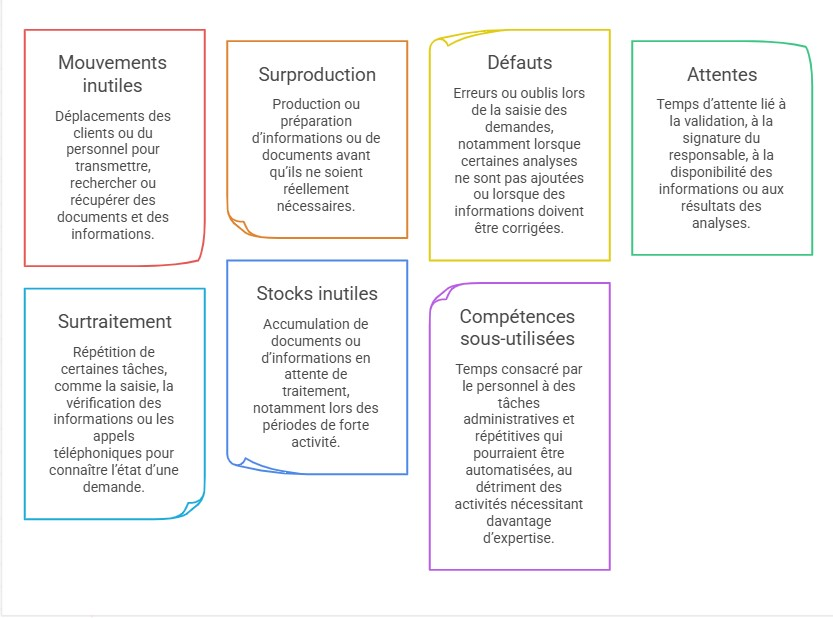
\includegraphics[width=0.85\textwidth]{muda-ctaa.jpg}
  \caption{Les sept Muda appliqués au fonctionnement du CTAA.}
  \label{fig:muda}
\end{figure}

Ces constats confirment la nécessité d'automatiser et de centraliser les processus afin de réduire les tâches à faible valeur ajoutée et d'accélérer le traitement des demandes.

\subsection{Solution proposée}

La solution proposée s'inscrit dans la transformation numérique du laboratoire, que l'on désigne souvent par le terme de « Laboratoire~4.0 ». Le déploiement d'un \ac{LIMS} en constitue l'élément central. Ce système permet de digitaliser et de centraliser les flux analytiques, de structurer les données du laboratoire et de suivre le cycle de vie de chaque échantillon, de sa réception jusqu'à l'émission du résultat validé. Il est complété par :
\begin{itemize}
    \item \textbf{une identification des échantillons par code \ac{QR}} dans le module de gestion des demandes : le code \ac{QR} contient davantage d'informations, se lit dans toutes les orientations et tolère une dégradation partielle de l'étiquette \citep{iso18004}. Les autres modules (réceptions, préparations, stocks) conservent pour l'instant le code-barres, dont la généralisation vers le code \ac{QR} constitue une perspective ;
    \item \textbf{un module de traçabilité} qui, à partir de la lecture d'un code ou de la saisie d'un numéro de série, reconstitue l'historique des opérations associées ;
    \item \textbf{le portail client} du \ac{CTAA}, qui permet aux clients de déposer leurs demandes et de consulter leurs rapports à distance.
\end{itemize}

Le tableau~\ref{tab:comparatif-lims} compare le fonctionnement du laboratoire avant et après le déploiement du \ac{LIMS}.

\begin{table}[H]
\centering
\renewcommand{\arraystretch}{1.25}
\begin{tabularx}{\textwidth}{|p{3.4cm}|Y|Y|}
\hline
\enteteligne \entete{Critère} & \entete{Avant le LIMS} & \entete{Après le LIMS} \\ \hline
Gestion des échantillons & Documents papier, gestion manuelle & Gestion numérique et centralisée \\ \hline
Identification & Code-barres linéaire, saisies manuelles & Code QR pour les échantillons, lecture par douchette \\ \hline
Saisie des données & Ressaisies, risque d'erreur élevé & Saisie unique, contrôles automatiques \\ \hline
Traçabilité & Limitée et dispersée & Historique numérique des opérations \\ \hline
Recherche d'information & Consultation successive de plusieurs documents & Recherche ou scan d'un identifiant \\ \hline
Suivi des demandes & Déplacements ou appels des clients & Suivi en ligne via le portail client \\ \hline
Équipements et habilitations & Suivi manuel des échéances & Suivi centralisé de la métrologie et des habilitations \\ \hline
Sécurité des données & Risque de perte ou de modification & Droits d'accès par rôle et historisation \\ \hline
Prise de décision & Informations peu disponibles & Données centralisées et exploitables \\ \hline
\end{tabularx}
\caption{Comparaison du fonctionnement du CTAA avant et après le déploiement du LIMS.}
\label{tab:comparatif-lims}
\end{table}

\subsubsection*{Évaluation du retour sur investissement}

Les gains économiques ont été estimés selon une méthode en quatre temps, détaillée dans l'annexe~\ref{annexe:gains} : identification des sources de gain, quantification des volumes, estimation du temps gagné par opération, puis valorisation au coût horaire chargé. Deux scénarios encadrent l'incertitude : un scénario \emph{prudent} et un scénario \emph{optimiste}. Le tableau~\ref{tab:gains-ctaa} présente le résultat.

\begin{table}[H]
\centering
\renewcommand{\arraystretch}{1.25}
\begin{tabularx}{\textwidth}{|p{3.6cm}|Y|r|r|}
\hline
\enteteligne \entete{Source de gain} & \entete{Description} & \entete{Prudent} & \entete{Optimiste} \\ \hline
Traitement des demandes & Moins de saisie et de gestion manuelle des demandes & 18\,750 & 25\,000 \\ \hline
Recherche des échantillons & Localisation et identification plus rapides & 22\,500 & 22\,500 \\ \hline
Archivage & Moins de classement et de stockage physique & 3\,000 & 3\,000 \\ \hline
Réduction des erreurs & Moins d'erreurs de saisie et de transcription & 1\,500 & 1\,500 \\ \hline
Consommation de papier & Dématérialisation des documents & 1\,200 & 1\,200 \\ \hline
\rowcolor{bleuclair} \multicolumn{2}{|l|}{\textbf{Gain total annuel estimé (TND/an)}} & \textbf{46\,950} & \textbf{53\,200} \\ \hline
\end{tabularx}
\caption{CTAA : estimation des gains économiques annuels (en TND/an).}
\label{tab:gains-ctaa}
\end{table}

À partir de ces gains et d'un investissement initial de 60\,000~\ac{TND}, nous calculons deux indicateurs. Le \textbf{délai de récupération} (en mois) et le \textbf{\ac{ROI} sur trois ans} sont donnés par :
\[
\text{Délai} = \frac{I_0}{G_{\text{an}}} \times 12
\qquad\qquad
\text{ROI}_{3\,\text{ans}} = \frac{3\,G_{\text{an}} - I_0}{I_0} \times 100
\]
où $I_0$ est l'investissement initial et $G_{\text{an}}$ le gain annuel. Nous retenons un horizon de trois ans, car un \ac{LIMS} est un investissement durable dont les gains s'étalent sur plusieurs années. Le calcul suppose qu'aucun coût récurrent supplémentaire n'est ajouté ; l'annexe~\ref{annexe:gains} étudie la sensibilité du résultat à ce paramètre.

\begin{table}[H]
\centering
\renewcommand{\arraystretch}{1.25}
\begin{tabular}{|l|r|r|}
\hline
\enteteligne \entete{Indicateur} & \entete{Scénario prudent} & \entete{Scénario optimiste} \\ \hline
Gain annuel & 46\,950~TND & 53\,200~TND \\ \hline
Investissement initial & 60\,000~TND & 60\,000~TND \\ \hline
Délai de récupération & 15,3 mois & 13,5 mois \\ \hline
ROI sur 3 ans & 134,75\,\% & 166\,\% \\ \hline
\end{tabular}
\caption{Délai de récupération et ROI de la solution au CTAA.}
\label{tab:roi-ctaa}
\end{table}

Le délai de récupération dépasse légèrement un an : la première année ne suffit pas à rentabiliser l'investissement, mais celui-ci est largement amorti sur trois ans. Au-delà de ces gains chiffrables, le \ac{LIMS} apporte des bénéfices qualitatifs importants : meilleure traçabilité des échantillons et des analyses, données plus fiables, risque réduit de perte d'information et respect facilité des exigences de la norme \ac{ISO/CEI 17025}.

%-------------------------------------------------------------
\section{Deuxième cas d'étude : Pharmaghreb}
%-------------------------------------------------------------

\subsection{Présentation du cas}

Les Laboratoires Pharmaghreb ont été fondés en 1985 par M. Radhouane Bouzguenda, pharmacien, et se présentent comme la première industrie pharmaceutique privée de Tunisie \citep{pharmaghrebweb}. L'entreprise fabrique des médicaments et des produits parapharmaceutiques, produit sous licence et noue des partenariats industriels. Elle s'est étendue en Algérie en 2011 avec la création des laboratoires Pharmidal NS, et a obtenu en 2019 les certifications ISO~9001 (management de la qualité) et ISO~14001 (management environnemental). La qualité et la sécurité sont au cœur de son activité : elle applique les \ac{BPF} et assure la pharmacovigilance, c'est-à-dire la collecte, le suivi et l'évaluation des effets indésirables de ses médicaments.

\begin{figure}[H]
  \centering
  
\includegraphics[width=0.45\textwidth]{logo-pharmaghreb.jpg}
  \caption{Logo des Laboratoires Pharmaghreb.}
  \label{fig:pharmaghreb}
\end{figure}

Une industrie pharmaceutique enchaîne plusieurs étapes : fabrication, conditionnement, contrôle qualité, puis stockage avant distribution. Ses laboratoires de contrôle vérifient les caractéristiques des matières premières et des produits à chaque étape, à l'aide d'équipements de mesure de précision : balances analytiques, pH-mètres, titrateurs, polarimètres, spectromètres, etc. Notre étude a porté sur dix de ces équipements, principalement de marque Mettler Toledo ; leur liste et le résultat de leur étude figurent au chapitre~\ref{chap:realisation} (tableau~\ref{tab:etude-equipements}).

\subsection{Analyse de l'existant}

Ces équipements disposent de plusieurs interfaces de communication (\ac{RS-232}, Ethernet, USB), mais celles-ci ne sont pas exploitées : aucune solution ne transfère les mesures vers un système informatique centralisé. L'étude met en évidence les difficultés suivantes.

\subsubsection*{Difficultés liées aux mesures}
\begin{itemize}
    \item \textbf{Saisie manuelle des résultats} : l'opérateur lit la valeur sur l'équipement puis la recopie, ce qui provoque des erreurs de transcription et allonge le traitement.
    \item \textbf{Intégration limitée au système d'information} : les mesures restent sur l'équipement ou sont enregistrées à part, ce qui complique leur centralisation.
    \item \textbf{Traçabilité fragile} : sans association automatique entre la mesure, l'équipement, l'opérateur et l'horodatage, la reconstitution de l'historique est difficile, alors que les \ac{BPF} exigent l'intégrité des données de contrôle.
    \item \textbf{Exploitation limitée des données} : la dispersion des mesures complique leur consultation, leur archivage et leur réutilisation.
\end{itemize}

\subsubsection*{Difficultés liées à l'état des équipements}
\begin{itemize}
    \item \textbf{Visibilité limitée} : sans suivi en temps réel, l'état de fonctionnement des équipements est difficile à connaître.
    \item \textbf{Anticipation limitée des pannes} : sans suivi continu, les anomalies sont détectées tardivement et la maintenance est moins bien planifiée.
\end{itemize}

\subsection{Solution proposée}

Nous avons proposé une démarche de \emph{rétrofit} numérique inspirée de l'Industrie~4.0 \citep{lee2015} : plutôt que de remplacer les équipements, nous leur ajoutons des capacités de communication afin que leurs mesures soient collectées et transmises automatiquement aux systèmes numériques. La démarche comporte deux étapes :
\begin{enumerate}
    \item \textbf{l'étude de connectivité} de chaque équipement : interfaces disponibles, protocoles supportés (\ac{MT-SICS}, \ac{TCP}/\ac{IP}, \ac{FTP}) et tests de communication ;
    \item \textbf{la conception et la réalisation d'un module d'acquisition} pour les équipements qui ne disposent que d'une liaison série : un boîtier fondé sur un microcontrôleur ESP8266 récupère les mesures d'une balance par \ac{RS-232}, identifie l'opérateur par badge \ac{NFC} et transmet les données par \ac{Wi-Fi}.
\end{enumerate}

À terme, la collecte continue des données prépare la \emph{maintenance prédictive}, qui repose sur la surveillance des paramètres de fonctionnement et l'analyse de leur historique pour détecter les signes précurseurs de défaillance \citep{mobley2002}.

\textbf{Périmètre de la mission.} L'étude de connectivité a été menée sur dix équipements. Le module d'acquisition a été conçu, réalisé et testé avec succès sur une balance Mettler Toledo XSR205 : il s'agit d'un \textbf{prototype complet et fonctionnel, en attente de déploiement} sur site. Son intégration au système d'information et la connexion des autres équipements constituent les perspectives du projet.

\subsubsection*{Estimation des gains économiques annuels}

Les gains attendus ont été estimés avec la même méthode que pour le \ac{CTAA} (annexe~\ref{annexe:gains}). Ils proviennent de la suppression des saisies manuelles, de la baisse des erreurs, de la centralisation des données et de l'amélioration de la disponibilité des équipements (tableau~\ref{tab:gains-pharmaghreb}). Il s'agit d'une \textbf{approximation} : le coût de déploiement n'étant pas encore arrêté, le \ac{ROI} réel sera calculé lors du déploiement.

\begin{table}[H]
\centering
\renewcommand{\arraystretch}{1.25}
\begin{tabularx}{\textwidth}{|p{3.8cm}|Y|r|r|}
\hline
\enteteligne \entete{Source de gain} & \entete{Description} & \entete{Prudent} & \entete{Optimiste} \\ \hline
Réduction des saisies manuelles & Moins de temps consacré à la recopie des mesures & 12\,000 & 15\,000 \\ \hline
Réduction du temps de collecte & Acquisition automatique des données & 10\,000 & 12\,500 \\ \hline
Disponibilité des équipements & Détection plus précoce des anomalies & 7\,500 & 7\,500 \\ \hline
Centralisation des données & Moins de recherche et de consolidation & 5\,000 & 5\,000 \\ \hline
Réduction des erreurs de saisie & Moins d'erreurs de transcription & 2\,000 & 2\,000 \\ \hline
\rowcolor{bleuclair} \multicolumn{2}{|l|}{\textbf{Gain total annuel estimé (TND/an)}} & \textbf{36\,500} & \textbf{42\,000} \\ \hline
\end{tabularx}
\caption{Pharmaghreb : estimation approximative des gains économiques annuels (en TND/an).}
\label{tab:gains-pharmaghreb}
\end{table}

%-------------------------------------------------------------
\section{Problématique et objectifs}
%-------------------------------------------------------------

Les deux cas d'étude révèlent un constat commun : dans les laboratoires, la saisie manuelle, la dispersion des données et le manque de suivi pénalisent la fiabilité, la rapidité et la traçabilité des résultats. La problématique générale du projet se formule ainsi :

\begin{quote}
\emph{Comment digitaliser les processus analytiques d'un laboratoire, de la gestion des échantillons jusqu'aux machines connectées, tout en garantissant la fiabilité et la traçabilité des données ?}
\end{quote}

Elle se décline en deux questions, une par cas d'étude :
\begin{itemize}
    \item \textbf{\ac{CTAA}} : comment centraliser la gestion des échantillons et garantir leur traçabilité grâce à un \ac{LIMS} et à un module dédié ?
    \item \textbf{Pharmaghreb} : comment connecter des équipements d'analyse existants au système d'information afin d'automatiser la remontée des mesures ?
\end{itemize}

Pour y répondre, le projet poursuit les objectifs suivants :
\begin{enumerate}
    \item paramétrer et mettre en service le \ac{LIMS} au \ac{CTAA} ;
    \item concevoir et développer un module de traçabilité par code et par numéro de série ;
    \item former et accompagner les utilisateurs afin de garantir l'adoption de la solution ;
    \item étudier la connectivité des équipements de Pharmaghreb ;
    \item concevoir, réaliser et tester un prototype d'acquisition automatique des mesures ;
    \item préparer le déploiement de la solution et l'évolution vers la supervision et la maintenance prédictive.
\end{enumerate}

%-------------------------------------------------------------
\section{Méthodologie de gestion du projet}
%-------------------------------------------------------------

Le choix d'une méthodologie dépend de la nature du projet, de la taille de l'équipe, des délais et du niveau d'exigence. Les méthodes agiles comme Scrum ou Kanban privilégient la souplesse et les livraisons fréquentes, tandis que le cycle en V repose sur un enchaînement rigoureux de phases, chacune associée à une phase de vérification \citep{forsberg1991}.

Nous avons retenu le \textbf{cycle en V} (figure~\ref{fig:cycle-v}). Sa branche descendante va de l'expression des besoins à la réalisation, en passant par les spécifications et la conception. Sa branche montante regroupe les vérifications : chaque phase de conception y a son équivalent de test, des tests unitaires jusqu'à la recette.

\begin{figure}[H]
\centering
\begin{tikzpicture}[node distance=0.4cm]
  \node[bloc=3.4cm] (b) at (0,0)      {Expression des besoins\\{\scriptsize (chapitre~\ref{chap:cadre-general})}};
  \node[bloc=3.4cm] (s) at (1,-1.5)   {Spécification\\{\scriptsize (chapitre~\ref{chap:analyse-besoins})}};
  \node[bloc=3.4cm] (g) at (2,-3.0)   {Conception générale\\{\scriptsize (chapitre~\ref{chap:conception})}};
  \node[bloc=3.4cm] (d) at (3,-4.5)   {Conception détaillée\\{\scriptsize (chapitre~\ref{chap:conception})}};
  \node[blocvert=3.4cm] (r) at (6,-6.0) {Réalisation\\{\scriptsize (chapitre~\ref{chap:realisation})}};
  \node[blocorange=3.4cm] (u) at (9,-4.5)  {Tests unitaires};
  \node[blocorange=3.4cm] (i) at (10,-3.0) {Tests d'intégration};
  \node[blocorange=3.4cm] (v) at (11,-1.5) {Validation fonctionnelle};
  \node[blocorange=3.4cm] (c) at (12,0)    {Recette et mise en service};
  \draw[fleche] (b) -- (s); \draw[fleche] (s) -- (g); \draw[fleche] (g) -- (d);
  \draw[fleche] (d) |- (r); \draw[fleche] (r) -| (u);
  \draw[fleche] (u) -- (i); \draw[fleche] (i) -- (v); \draw[fleche] (v) -- (c);
  \draw[doublefleche, dashed, draw=gris!60] (b) -- (c);
  \draw[doublefleche, dashed, draw=gris!60] (s) -- (v);
  \draw[doublefleche, dashed, draw=gris!60] (g) -- (i);
  \draw[doublefleche, dashed, draw=gris!60] (d) -- (u);
\end{tikzpicture}
\caption{Le cycle en V appliqué au projet.}
\label{fig:cycle-v}
\end{figure}

Ce choix se justifie par plusieurs raisons :
\begin{itemize}
    \item un déroulement séquentiel, où chaque phase est terminée et validée avant la suivante ;
    \item une documentation détaillée à chaque étape, qui sert de référence tout au long du projet ;
    \item une traçabilité des exigences, de leur formulation jusqu'aux tests de validation ;
    \item une adéquation aux environnements réglementés, dont les besoins sont bien définis, comme les laboratoires accrédités et l'industrie pharmaceutique.
\end{itemize}

Nous avons toutefois assoupli ce cadre lors de la mise en service du \ac{LIMS} : les retours des utilisateurs recueillis pendant la formation ont donné lieu à de courtes boucles d'ajustement du paramétrage, sans remettre en cause les phases déjà validées.

%-------------------------------------------------------------
\section{Planification du projet}
%-------------------------------------------------------------

Le projet s'est déroulé de février à septembre 2026. Le diagramme de Gantt de la figure~\ref{fig:gantt} présente l'enchaînement des tâches des deux volets. Le volet Pharmaghreb a démarré pendant la phase de formation au \ac{CTAA}, ce qui explique le chevauchement des deux missions.

% À VÉRIFIER : ajuster les dates des tâches au déroulement réel du stage.
\begin{figure}[H]
\centering
\resizebox{\textwidth}{!}{%
\begin{ganttchart}[
    hgrid, vgrid={*1{draw=black!12}},
    x unit=0.62cm, y unit chart=0.58cm, y unit title=0.6cm,
    title/.append style={fill=bleu, draw=bleu},
    title label font=\footnotesize\color{white}\bfseries,
    bar/.append style={fill=bleu!55, draw=bleu},
    bar height=0.55, bar label font=\footnotesize,
    group/.append style={fill=bleu, draw=bleu}, group label font=\footnotesize\bfseries,
    group peaks height=0.2, group top shift=0.35, group height=0.25,
    milestone/.append style={fill=orange, draw=orange}, milestone label font=\footnotesize\itshape,
  ]{1}{16}
  \gantttitle{2026}{16} \\
  \gantttitle{Fév.}{2} \gantttitle{Mars}{2} \gantttitle{Avr.}{2} \gantttitle{Mai}{2}
  \gantttitle{Juin}{2} \gantttitle{Juil.}{2} \gantttitle{Août}{2} \gantttitle{Sept.}{2} \\
  \ganttgroup{Volet CTAA}{1}{14} \\
  \ganttbar{Intégration et étude de l'existant}{1}{2} \\
  \ganttbar{Spécification des besoins}{2}{3} \\
  \ganttbar{Paramétrage du LIMS}{3}{6} \\
  \ganttbar{Étiquetage (codes-barres et codes QR)}{6}{8} \\
  \ganttbar{Formation et accompagnement}{8}{10} \\
  \ganttmilestone{Mise en service du LIMS}{10} \\
  \ganttbar{Conception du module de traçabilité}{11}{12} \\
  \ganttbar{Développement du module}{12}{14} \\
  \ganttbar{Tests et validation du module}{14}{14} \\
  \ganttgroup{Volet Pharmaghreb}{9}{16} \\
  \ganttbar{Étude des équipements et protocoles}{9}{11} \\
  \ganttbar{Tests de communication}{11}{12} \\
  \ganttbar{Conception du prototype}{13}{14} \\
  \ganttbar{Réalisation et tests du prototype}{14}{16} \\
  \ganttgroup{Transverse}{14}{16} \\
  \ganttbar{Rédaction du rapport}{14}{16}
\end{ganttchart}}
\caption{Diagramme de Gantt du projet.}
\label{fig:gantt}
\end{figure}

%-------------------------------------------------------------
\section*{Conclusion}
\addcontentsline{toc}{section}{Conclusion}
%-------------------------------------------------------------

Ce chapitre a présenté le contexte général du projet et les organismes concernés. Nous avons analysé l'existant des deux cas d'étude, le \ac{CTAA} et Pharmaghreb, mis en évidence leurs principales difficultés et présenté les solutions numériques proposées, ainsi que leur intérêt économique. Nous avons ensuite formulé la problématique et les objectifs, puis présenté la méthodologie et la planification du projet. Le chapitre suivant est consacré à l'analyse et à la spécification des besoins.
